\documentclass[a4paper, 11pt, ngerman, fleqn]{article}
\usepackage[utf8]{inputenc}
\usepackage{babel}
\usepackage{ngerman}
\usepackage{coordsys,logsys,color}
\usepackage{german,fancyhdr}
\usepackage{hyperref}
\usepackage{texdraw}				
\usepackage[T1]{fontenc}					
\usepackage{amsmath,amsfonts,amssymb}	
\usepackage[normalem]{ulem}	
\usepackage{listings}
\usepackage{graphicx}


\hypersetup{colorlinks=true, breaklinks=true, linkcolor=darkblue, menucolor=darkblue, urlcolor=darkblue, citecolor=darkblue}

\lhead{\sc{Reviewdokument: Real Time Mesh Utilities}}

\pagestyle{fancy}


%%%DOCUMENTCLASS%%%
\documentclass[a4paper, 12pt, english, fleqn]{article}


%%%USEPACKAGES%%%
\usepackage[utf8]{inputenc}
\usepackage{babel}
\usepackage{coordsys,logsys,color}
\usepackage{fancyhdr}
\usepackage{hyperref}
\usepackage{texdraw}				
\usepackage[T1]{fontenc}					
\usepackage{amsmath,amsfonts,amssymb}	
\usepackage[normalem]{ulem}	
\usepackage{listings}
\usepackage{graphicx}
\usepackage{enumitem}
\usepackage[paper=a4paper,left=35mm,right=35mm,top=35mm,bottom=30mm]{geometry}

%%%PAGESTYLE%%%
\pagestyle{fancy}


%%%LINKING%%%
\hypersetup{colorlinks=true, breaklinks=true, linkcolor=blue, menucolor=darkred, urlcolor=darkblue, citecolor=darkblue}

%%%NEWLIST%%%    Itemnamen bold, Text eingerückt 
\newlist{aims}{enumerate}{1}
\setlist[aims,1]{
	label={Aim~\arabic*},
	leftmargin=*,
	align=left,
	%labelsep=1mm,
	font=\bfseries
}

%%%NEWCOMMAND%%%
\newcommand{\titlefont}[1]{\textcolor{black}{\fontseries{bx}\fontshape{n}\fontsize{30}{0pt} \selectfont #1}}
\newcommand{\titlepagef}[1]{\textcolor{black}{\fontseries{bx}\fontshape{n}\fontsize{14}{0pt} \selectfont #1}}
\newcommand{\gloss}[1]{\textcolor{glossb}{\fontsize{11}{0pt}\selectfont #1}}
\newcommand{\spaceline}[1][8pt]{\vskip #1}
\newcommand{\attrname}[1]{\textcolor{fgcgray}{\scriptsize #1}}
\newcommand{\comment}[1]{\spaceline[5pt] \textcolor{fgcgray}{\scriptsize #1} \spaceline[15pt]}


%%%RENEWCOMMAND%%%
\renewcommand{\familydefault}{cmss}


%%%DEFINECOLOR%%%
\definecolor{fgcgray}{rgb}{0.4, 0.4, 0.4}
\definecolor{darkred}{rgb}{.6,0,0}
\definecolor{glossb}{rgb}{0,0,0.38}


%%%LENGTH SETTINGS%%%
\addtolength{\oddsidemargin}{-1.0cm}
\addtolength{\evensidemargin}{-1.0cm}
\addtolength{\headwidth}{2.0cm}
\addtolength{\textwidth}{2.0cm}

\setlength{\parindent}{0cm}


%%%DEFINITIONS%%%
%Füge Überschriften ein
%Füge Namen ein

\makeatletter

\def\@maketitle{
	%\begin{titlepage}
	
	\begin{center}
		\titlepagef{Software-Project 2017}
		\spaceline
	\end{center}
	
	\begin{center}
		\parbox{\textwidth}{
			\spaceline
			\centering{\titlefont{\@title}}
			\par
			\spaceline
		}
	\end{center}
	
	\begin{center}
		\titlepagef{Real-Time Mesh Utilities}
		\spaceline[2em]
	\end{center}
	
	\begin{center}
		\begin{tabbing}
			Petros Simidyan \qquad \=
			Blerta Hamzallari \qquad \=
			Felix Griesau \qquad \=
			Marco Klamke \\
			Julius Lerm
			\>Lars Debor
			\>Simon Heinke  
			\>Sugandha Sachdeva
		\end{tabbing}
	\end{center}
	
	\spaceline[3em] {
		\begin{flushright}
			\begin{tabular}[t]{rl}
				\attrname{last change:} & \@date
			\end{tabular}
		\end{flushright}
		\par
	}
	\spaceline[5.5em]
	%\end{titlepage}
}

\makeatother


\begin{document}
\title{Review Document: Real Time Mesh Utilities}
\vspace{3 in}
\maketitle
\clearpage

\section*{Review Document}
The review document is divided into two parts.
It contains the results of planning as well as the outcomes of the design process.
Results of planning include development model, cost and risk estimation, milestones and organization.
The design process contains the outcomes of the current iteration, arrangements for the next iteration and a list of tools.



\subsection{Result of Planning}
A large part of the first phase of the project (i.e. scheduling and draft) is reflected on the functional specification document. The requirement analysis is registered, the objectives are declared, whereas the decisions and the product information is written down.

\subsubsection{Software Development Model}

This section contains information about the software model chosen, based on the requirements of the project.
The principals of the group, client requirement and knowledge about the project play an important role in choosing the development model. Based on the latter, the development team decides its work flow. 

\begin{aims}
	\leftskip=0,8cm
	\item[Agile Development Model: SCRUM] The group chose SCRUM because it is an iterative and incremental agile software development framework for managing product development. The duration of each sprint was set to two weeks. Each phase of the software development has two sprints. 
	
	Every sprint ends with a presentation by the relevant working group about the developments and progress during the sprint. The end of the respective phase of the project is marked by a working prototype and a presentation which includes a summary of the work done by the entire team. 
	
	\item[Projects specific adaptation to the model:] Every person in the team has multiple roles. All group members work on both the document and the code.
\end{aims} 

\paragraph{Software Development Specific Content}
Since the group decided for the agile development project, the milestones need to be stated and agreed upon by the team. Milestones are the aim or the expected output of each development phase. They help the team to specify what features should be completed by which deadline.

\newpage

\subsubsection{Effort Estimate}
The main purpose in the effort estimation section is the categorization of the different parts of the project regarding their complexity and effort criteria.  
 (see figure 1)

\begin{figure}[h]
	\begin{center}
		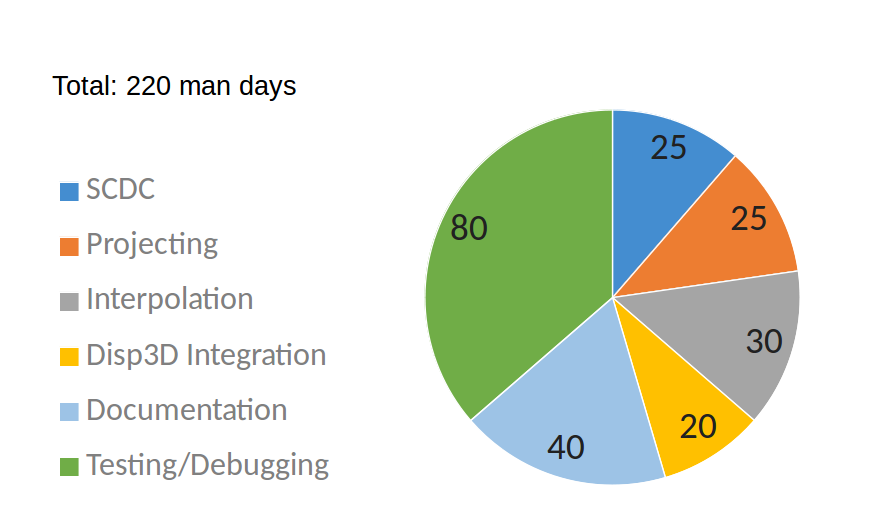
\includegraphics[width= 14cm]{figures/aufwandsabschaetzung.png}
		\caption{Effort estimate}
	\end{center}
\end{figure}

\clearpage

\subsubsection{Risk Estimate}
In this section, the probabilities of the different risks involved in the project are listed. This will help the team to determine what aspects of the implementation should get a higher priority.

\begin{description}
	\item[RE1:] Communication problems in the team
	\item[RE2:] Coverage is too extensive
	\item[RE3:] Framework does not provide the needed functionality 
	\item[RE4:] Resource bottleneck derived from team members temporary absence 
	\item[RE5:] Change of the requirements due to miscommunication with the product owner 
	\item[RE6:] Hidden complexity 
	\item[RE7:] Acceptable computation time takes a lot more effort than expected  
\end{description}

\begin{figure}[h]
	\begin{center}
		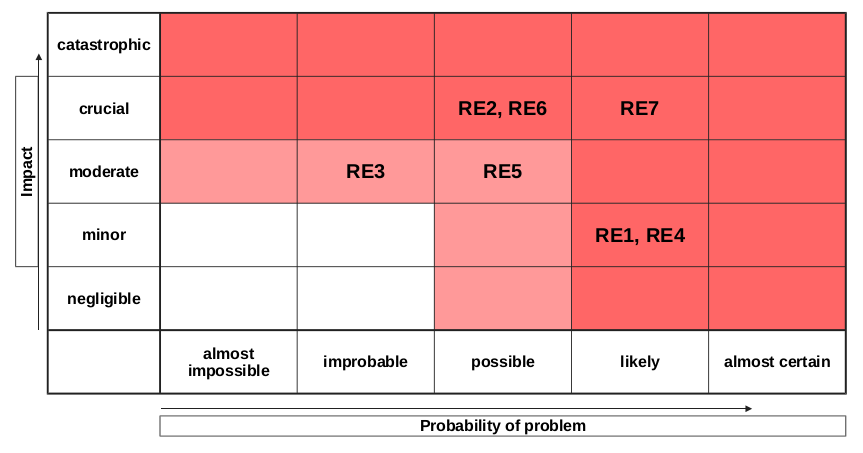
\includegraphics[width= 15cm]{figures/risikoabschaetzung.png}
		\caption{Risk estimate}
	\end{center}
\end{figure}

\paragraph{Handling Risks}

In case one of the risks occurs, certain strategies for solving the issue are provided. Only the ones having a crucial impact on the project are dealt with in the following section. 

\begin{aims}
	
	\item[RE2:]Optional requirements will only be addressed after every mandatory criteria is fulfilled.
	\item[RE6:]The team communicates with the product owners to eradicate all ambiguities.
	\item[RE7:]To keep the computation time as low as possible, changes to the software will be tested constantly to 						   determine even minor impacts on efficiency. 	
	
\end{aims}

\clearpage

\subsubsection{Milestones} 
These Milestones provide major dates for significant events during the time of the project. Furthermore they serve as a guideline for the progress that is desired at a certain point of the development process.
~\\
~\\

\begin{tabular}{lll}
 	\textbf{First Phase} & 03.05.2017 & First Phase Finished\\
	\textbf{Second Phase} & 04.06.2017 & Detailed Design and Features Implemented\\
				& 08.06.2017 & Second Phase Finished\\
	\textbf{Third Phase} & 21.06.2017 & Features Tested and Optimized\\          
				& 02.07.2017 & Portation to MNE Scan\\
				& 05.07.2017 & End of Project\\
\end{tabular}

~\\

\begin{figure}[h]
	\begin{center}
		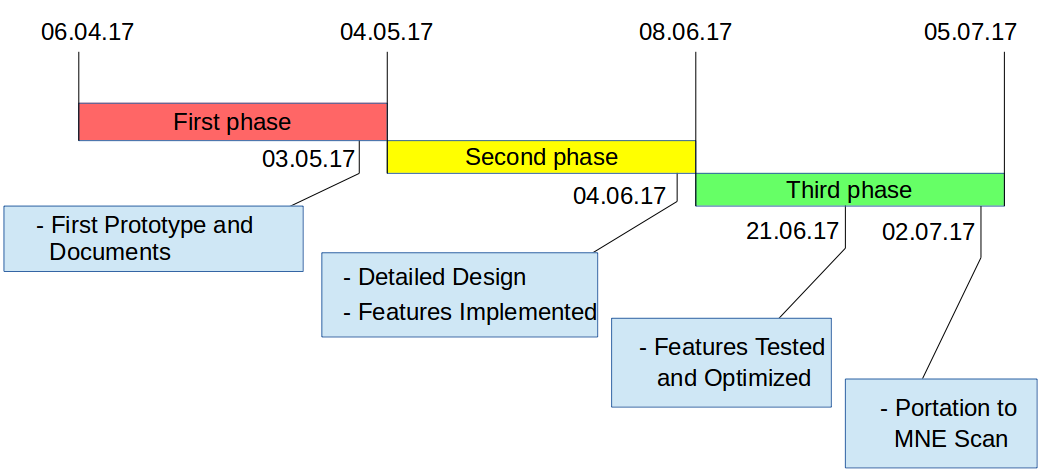
\includegraphics[width= 15cm]{figures/milestones_timeline.png}
		\caption{Timeline of milestones}
	\end{center}
\end{figure}

\paragraph{Checklist}
\begin{aims}
	\item[03.05.2017]First Phase Finished
	\begin{enumerate}\itemsep0pt 
		\item Functional Specification
		\item Preliminary Design
		\item Review Document
		\item First Prototype
		\item Presentation
	\end{enumerate}
	
	\item[04.06.2017]Detailed Design and Features Implemented
	\begin{enumerate}\itemsep0pt
		\item Detailed Design
		\item SCDC (operational)
		\item Projecting Algorithm (operational)
		\item Interpolation Algorithm (operational)
	\end{enumerate}
	
	\item[08.06.2017]Second Phase Finished
	\begin{enumerate}\itemsep0pt
		\item Presentation
		\item Review Document
		\item Integration into Disp3D
	\end{enumerate}

	\item[21.06.2017]Features Tested and Optimized
	\begin{enumerate}\itemsep0pt
		\item SCDC (tested)
		\item Projecting Algorithm (tested)
	\end{enumerate}
	
	\item[02.07.2017]Portation to MNE Scan
	
	\item[05.07.2017]End of Project
	\begin{enumerate}\itemsep0pt
		\item Review Document
		\item Presentation
		\item Interpolation Optimized
	\end{enumerate}


\end{aims}

\newpage

\subsubsection{Organization}

This section concerns to the rules, agreements and the partitioning regarding the teamwork in the project, so the work itself will be efficient and organized. 

\paragraph{Ways of Communication}
\begin{aims}
	\item[Telegram:] Used for quick and direct team communication so that possible misunderstandings will be solved in no time.
	
	\item[E-mail distribution list:] Used for scheduling the team meetings and communications with the extended team, including the product owners. 
	
	\item[Team meetings:] Used for the review and direct discussion of the encountered problems. 
	
	\item[Skype:] Used in the cases of the absence of a team member. 
	
	\item [Jira:] Used for scheduling tasks and keeping track of the progress done by each member of the team.
	
	\item[Dropbox:] Used for exchanging documents and file sharing.  
\end{aims}

\paragraph{Additional Agreements}
\begin{itemize}
	\item Internal team meetings (without product owners): Tuesdays and Thursdays at 19:00
	
	\item External team meeting (with the product owners): Wednesdays at 17:00
	
	\item Meeting of subgroups : upon consultation and demand 
\end{itemize}

\paragraph{Role Assignment in SCRUM}

\begin{aims}
	\leftskip=0,8cm
	\item[Product Owner:] Thomas Jochmann, Lorenz Esch
	
	\item[Scrum Master:] Simon Heinke
	
	\item[Development team:] Blerta Hamzallari, Felix Griesau, Julius Lerm, Lars Debor, Marco Klamke, Simon Heinke, Sugandha Sachdeva, Petros Simidyan
	
	\item[Client, User:] Participants of the MNE CPP project of Boston Children's Hospital
	
\end{aims}

\paragraph{Role Assignment Organization}
\begin{aims}
	\leftskip=0,8cm
	\item[Advisor:] Thomas Jochmann, Lorenz Esch
	
	\item[Team leader:] Simon Heinke
	
	\item[Build master:] Lars Debor
	
	\item[Version management:] Felix Griesau
	
\end{aims}

\clearpage
\section{Ergebnisse des Entwurfs}

Die Ergebnisse des Entwurfs sind zum größten Teil in der Entwurfsdokumentation nachzulesen.
Dort sind die Zusammenhänge der verschiedenen Pakete, Komponenten und Klassen aufgezeigt und anschaulich mit Hilfe von UML-Diagrammen dargestellt.

\subsection{Werkzeuge} 

Die verwendeten Werkzeuge sind Softwarelösungen, die die einzelnen Bereiche der Organisation und Entwicklung ermöglichen bzw. erleichtern.

\subsubsection{Organisatorische Werkzeuge}
	\begin{description}
		\item[Phabrikator:] Zuweisung einzelner, zu bearbeitender Tasks und deren Verwaltung, sowie die Bereitstellung des Wiki's. 
		
		\item[Quellcodeverwaltung:]	Hierfür wird \textit{Subversion} benutzt um einen einheitliche Arbeitsgrundlage an den Dateien zu gewährleisten.
		
		\item[Arbeitszeitenerfassung:] Hierfür wird \textit{Kimai} verwendet, dort werden alle Zeiten eingetragen und verschiedenen Themen/Bereichen zugeteilt.
		
		\item[LaTeX:] Hierbei handelt es sich um eine Textbeschreibungssprache, mit der verschiedenste Dokumente erstellt werden können. 
		Diese stehen nach der Erstellung in verschiedenen Formaten zur Verfügung.
		Im speziellen wird es in diesem Projekt für die Erstellung des Pflichtenheftes, den Reviewdokumenten und dem Entwurfsdokument verwendet.   
		
		\item[Doxygen:] Mit diesem Programm werden die Kommentare aus dem erstellten Code gezogen, um daraus eine Dokumentation der Implementierung zu erzeugen.
		
		\item[PlantUML:] Erzeugung von UML-Diagrammen, die Aktivitäten, Aufbau und Funktionen des Systems grafisch darstellen. 
	\end{description}

\subsubsection{Entwicklungswerkzeuge}
	\begin{description}
		\item[Buildsystem:] Es wird \textit{scons} verwendet um eine einheitliche und angepasste Kompilierung von C++-Dateien zu gewährleisten. 
		Hierbei werden sogenannte \textit{sconstruct} erstellt, mit denen verschiedene Vorbedingungen, wie das Einbinden von Bibliotheken und die Auswahl des Kompilers erfüllt werden können.
		
		\item[Entwicklungsumgebung:] Ein beliebiger \textit{Texteditor}, der Syntaxhighlighting für die Programmiersprache C++ unterstützt, wird zum Verfassen des Codes verwendet.
		
		\item[Programmiersprache:] Es wird die hardwarenahe Programmiersprache \textit{C++} verwendet, da diese alle, für das Projekt erforderlichen, Anforderungen erfüllt.
		
		\item[Betriebssystem:] Für den Betrieb der Software ist \textit{Linux} unabdingbar, da das verwendete DPDK-Framework nur auf dessen Grundlage funktioniert.
		
		\item[Bibliotheken:] In diesem Projekt werden viele verschiedene Standardbibliotheken von C++ und vom Auftraggeber bereitgestellte Bibliotheken verwendet. 
		Zusätzlich hierzu wird als spezielles Framework (Ansammlung von Bibliotheken) das DPDK genutzt. 
		Dieses liefert mit seiner umfangreichen Klassensammlung die Grundlage (Verschlüsselung, Forwarding, ...) für das System. 
		
	\end{description}

\subsection{Ergebnisse des Entwurfs für die erste Iteration:}
Die Ergebnisse der ersten Iteration ergeben sich aus dem aktuell zu erreichenden Meilenstein.

\begin{description}
	\leftskip=0,8cm
		\item[Pflichtenheft:] Das Lastenheft wurde vollständig in das Pflichtenheft überführt und um weitere Punkte, im Dialog mit dem Auftraggeber, ergänzt.
		
		\item[Grobentwurf:] Der Grobentwurf umfasst eine erste Übersicht über die Funktions- und Arbeitsweise des Systems.
		
		\item[Implementierung:] Eine erste Lauffähige Implementierung wurde umgesetzt und umfasst die Funktionen eines einfachen Forwardings ohne Verschlüsselung.
		
		\item[Planung:] Es wurden Festlegungen für die weiteren Iterationen getroffen, hierbei wurden insbesondere die Meilensteine für die nächste Iteration festgelegt und das weitere Vorgehen innerhalb des Teams besprochen.
		
	\end{description}

\subsection{Festlegungen für die nächste Iteration:}
Die Festlegungen für die jeweilige nächste Iteration spiegeln sich in den Meilensteinen wieder.

\begin{description}
	\leftskip=0,8cm
		\item[Grobentwurf verfeinern:] Der Grobentwurf wird um spezifischere Diagramme und Beschreibungen zum Feinentwurf ergänzt. Dies geschieht jeweils parallel zu den Meilensteinen, da automatisch jede Änderung dort festgehalten wird.
		
		\item[Implementierung erweitern:] Die aktuelle Implementierung wird um einen ersten Entwurf der Verschlüsselung mit statischem Schlüssel erweitert.
		
		\item[Hardware konfigurieren:] Die zur Verfügung gestellte Hardware wird initial konfiguriert um die Voraussetzungen für das System zu gewährleisten und um die Implementierung ersten Tests unterziehen zu können.
		
	\end{description}
  
\end{document}


	
